\newpage
%\pagestyle{empty}

\begin{minipage}[c]{.25\linewidth}
	
\includegraphics[width=4cm]{images/LEnsE_IOGS.jpg}
\end{minipage} \hfill
\begin{minipage}[c]{.4\linewidth}

\begin{center}
\vspace{0.3cm}
{\Large \textsc{Opto-Électronique}}

\medskip

5N-027-SCI \qquad \textbf{\Large TD Séance 1}

\end{center}
\end{minipage}\hfill

%%%%%%%%%%%%%%%%%%%%%%%%%%%%%%%%%%
\section{TD1 - Bases de l'électronique}

%%%%%%%%%%%%%%%%%%%%%%%%%%%%%%%%%%%%%%%%%%%%%%%%%%%%%%%
\subsection{Exercice 1 - Pont diviseur}

Soit le circuit suivant :

\begin{center}
\begin{circuitikz}
	\draw (1,0) to [short, *-] (3,0)
		to[R=$R_{2}$, -*, i<_=$I_2$] (3,2)
		to[R=$R_{1}$, -] (3,4)
		to [short, -o, i<_=$I$] (0,4);
	\draw (3,0) to[short, -o] (4,0);
	\draw[dashed] (4,0) to[short, -] (5.5,0) 
		to[R=$R_L$, -] (5.5,2)
		to[short, -] (4,2);
	\draw (3,2) to[short, -o, i=$I_S$] (4,2);
	
	% fleche
	\draw (0,0.5) edge[->] (0,3.5);
	\node (Ein) at (-1,2.25){$V_E$};

	\draw (0,0) to [short, o-] (1,0)
		node[ground](GND){};
	% fleche
	\draw (3.5,0.3) edge[->, green!40!black] (3.5,1.7); \node[text=green!40!black] (US) at (4,1){$V_S$};
\end{circuitikz}
\end{center}

\begin{enumerate}
	\item Donnez l'expression de $V_S$ en fonction de $V_E$.
	\item Quel est l'impact de la résistance de charge $R_L$ ?
\end{enumerate}

\subsection*{Réponse}

Si on suppose que $I_S = 0$ (pas de résistance $R_L$), on peut s'intéresser au courant $I$ en écrivant deux lois des mailles différentes :

\begin{enumerate}
	\item $V_E - R_1 \cdot I - R_2 \cdot I = 0$
	\item $V_S - R_2 \cdot I = 0$
\end{enumerate}

Cela suppose que l'on considère que le courant $I_S = 0$.

En combinant les deux, on obtient la relation entre $V_E$ et $V_S$ suivante : $$\boxed{V_S = V_E \cdot \frac{R_2}{R_1 + R_2}}$$

\noindent\hrulefill


Si on suppose maintenant que le circuit précédent est chargé par une résistance $R_L$, on obtient alors le montage suivant :

Dans ce cas, le courant $I_S$ n'est plus nul.

Le courant $I$ traversant $R_1$ va alors se partager entre $R_2$ et $R_L$. On aura alors la seconde loi des mailles écrites précédemment qui ne sera plus valide.

On peut alors écrire les relations suivantes :
\begin{enumerate}
	\item loi des mailles : $V_E - R_1 \cdot I + V_S$ 
	\item loi des mailles : $V_S - R_L \cdot I_S = 0$  
	\item loi des noeuds : $I = I_S + I_2$ 
	\item loi des mailles : $V_S - R_2 \cdot I_2 = 0$
\end{enumerate}

Après regroupement et simplification, on obtient la relation suivante : $$\boxed{V_S = V_E \cdot \frac{R_{eq}}{R_1 + R_{eq}}}$$  

avec $R_{eq} = \frac{R_2 \cdot R_L}{R_2 + R_L}$ (mise en parallèle de $R_2$ et $R_L$).

\newpage
%%%%%%%%%%%%%%%%%%%%%%%%%%%%%%%%%%%%%%%%%%%%%%%%%%%%%%%
\subsection{Exercice 2 - Courants et tensions}

Soit le circuit suivant :

\begin{center}
\begin{circuitikz}
\draw (0,0) to[I, l=$I_{PHD}$, invert] (0,3)
	to[short, -*, i=$I_{PHD}$] (2,3)
	to[R, R=$Z_{PHD}$, -*] (2,0)
	to[short] (0,0);
	
\draw (1,0) to[short, *-] (1,0) node[ground] {};
\draw (2,3) to[short, -*] (4,3) to[R, R=$R_{PHD}$, -*] (4, 0)
	-- (2,0);

\draw (4,3) to[short, -*] (6,3) to[R, R=$R_{e}$, -*] (6, 0)
	-- (4,0);

\draw (6,3) -- (8,3) to[R, R=$Z_{e}$] (8,0) -- (6,0);
\end{circuitikz}
\end{center}

\begin{enumerate}
	\item Donnez l'expression de $V_S$ en fonction de $I_{PHD}$.
	\item Que devient cette expression si $R_e \longrightarrow +\infty$, $Z_e \longrightarrow +\infty$ et $Z_{PHD} \longrightarrow +\infty$ ?
	
	\medskip 
	
	On se place à présent en régime harmonique.
	
	$Z_{PHD} $ est une capacité $C_{PHD} $ et $Z_e$ est une capacité $C_e$.
	
	\item Que devient l'expression de $V_S$ en fonction de $I_{PHD}$ ?
	\item A quoi peuvent correspondre l'ensemble des éléments du montage ?
	
\end{enumerate}

\subsection*{Réponse}

%%%%%%%%%%%%%%%%%%%
\textbf{Question 1}
	
Les 5 branches sont en parallèle et sont soumises à la même différence de potentiel $V_S$.

Le courant $I_{PHD}$ se distribue dans les 4 autres branches : $I_{PHD} = \frac{V_S}{Z_{PHD}} + \frac{V_S}{R_{PHD}} + \frac{V_S}{Z_{e}} + \frac{V_S}{R_{e}}$

Ainsi : $$V_S = \frac{I_{PHD}}{\frac{1}{Z_{PHD}} + \frac{1}{R_{PHD}} + \frac{1}{Z_{e}} + \frac{1}{R_{e}}}$$


\textbf{Question 2}

L'expression précédente devient : $V_S = R_{PHD} \cdot I_{PHD}$

\textbf{Question 3}

$Z_{PHD} = \frac{1}{j \cdot C_{PHD} \cdot \omega}$ et $Z_{e} = \frac{1}{j \cdot C_{e} \cdot \omega}$ 

L'expression de la question 1 devient alors : $$\frac{V_S}{I_{PHD}} = \frac{1}{\frac{1}{R_{PHD}} + j \cdot C_{PHD} \cdot \omega + \frac{1}{R_{e}} + j \cdot C_{e} \cdot \omega}$$

On pose : $R_k = \frac{R_e \cdot R_{PHD}}{R_e + R_{PHD}}$ et $C_k = C_{PHD} + C_e$

Après simplification : $$\frac{V_S}{I_{PHD}} = R_k \cdot \frac{1}{1 + j \cdot R_k \cdot C_k \cdot \omega}$$

\textbf{Question 4}
	
Une \textbf{photodiode} peut être modélisée par une source de courant, dépendant du flux lumineux qu'elle reçoit, et d'une capacité parasite $C_{PHD}$.

De l'autre côté, il est possible de modéliser un oscilloscope, permettant de visualiser le signal électrique, par une résistance d'entrée $R_e$ et le cable coaxial, qui permet d'amener le signal jusqu'à l'entrée de l'oscilloscope, par un condensateur de capacité $C_e$.

Enfin, la résistance $R_{PHD}$ permet de transformer le courant résultant de la photodiode en une tension plus facilement visualisable à  l'aide d'un oscilloscope.


\newpage
%%%%%%%%%%%%%%%%%%%%%%%%%%%%%%%%%%%%%%%%%%%%%%%%%%%%%%%
\subsection{Exercice 3 - Charge et décharge d'un condensateur}

Soit le circuit suivant :

\begin{center}
\begin{circuitikz}
	\draw (0,0) to [R=$R$, o-*] (3,0)
		to[C=$C$, -*] (3,-3)
		to[short, -*](1,-3)
		node[ground](GND){}
		to[short, -o](0,-3);
	\draw (3,0) to[short, -o](4,0);
	\draw (3,-3) to[short, -o](4,-3);
	% fleche
	\draw (0,-2.7) edge[->] (0,-0.3);
	\node (Ein) at (-0.5,-1.5){$V_E$};
	% fleche
	\draw (4,-0.3) edge[<-, green!40!black] (4,-2.7); 
	\node[text=green!40!black] (US) at (4.5,-1.5){$V_S$};
\end{circuitikz}
\end{center}

\begin{enumerate}
	\item Donnez le lien entre $V_E(t)$ et $V_S(t)$.
	\item Donnez l'expression de $V_S(t)$ pour $t > 0$ pour $V_E(t) = E$ (constante). On supposera le condensateur totalement déchargé à $t = 0$ (c'est à dire si $V_S(0) = 0$) et tracez $V_S(t)$.
	\item Donnez le protocole de mesure de la \textbf{réponse indicielle} de ce circuit. 
\end{enumerate}

\subsection*{Réponse}

\textbf{Question 1}

La loi des mailles donne : $V_E(t) - R \cdot i(t) - V_S(t) = 0$ et la caractéristique d'un condensateur donne : $i(t) = C \cdot \frac{d V_S(t)}{d t}$.

En effet, pour un condensateur : $q = C \cdot V_S (t)$ et le courant associé vaut alors $i = \frac{d q}{d t}$

Ainsi : 

$$V_E(t) = R \cdot C \cdot \frac{d V_S(t)}{d t} + V_S(t)$$

\centerline {\rule{.5\linewidth}{.25pt}} % Horizontal line

\textbf{Question 2}

a) On cherche les solutions de l'équation homogène : $$\frac{d V_S(t)}{d t} + \frac{1}{R \cdot C} \cdot V_S(t) = 0$$

Ces solutions sont de la forme : $V_{S0}(t) = k \cdot exp(\frac{-t}{R \cdot C})$ avec $k \in \mathbb{R}$

b) On cherche une solution particulière de la même forme que le second membre. Dans notre cas, $E/RC$ qui est une constante.

Si $V_{S1}(t) = m$, alors $\frac{d V_{S1}(t)}{d t} = 0$.

On a alors, en reprenant l'équation initiale : $\frac{m}{R \cdot C} = \frac{E}{R \cdot C}$. Ainsi $m = E$.

c) Les solutions de l'équation sont alors la somme des deux solutions précédentes. Ainsi : $$V_S(t) = V_{S0}(t) + V_{S1}(t) = k \cdot exp(\frac{-t}{R \cdot C} + E$$

d) On obtient ensuite $k$ en utilisant la condition initiale, à savoir $V_S(0) = 0$. Ainsi $k = -E$.

On obtient alors l'expression suivante pour $V_s(t)$ :

$$V_S(t) = E \cdot (1 - exp(\frac{-t}{R \cdot C})$$

\begin{center}
	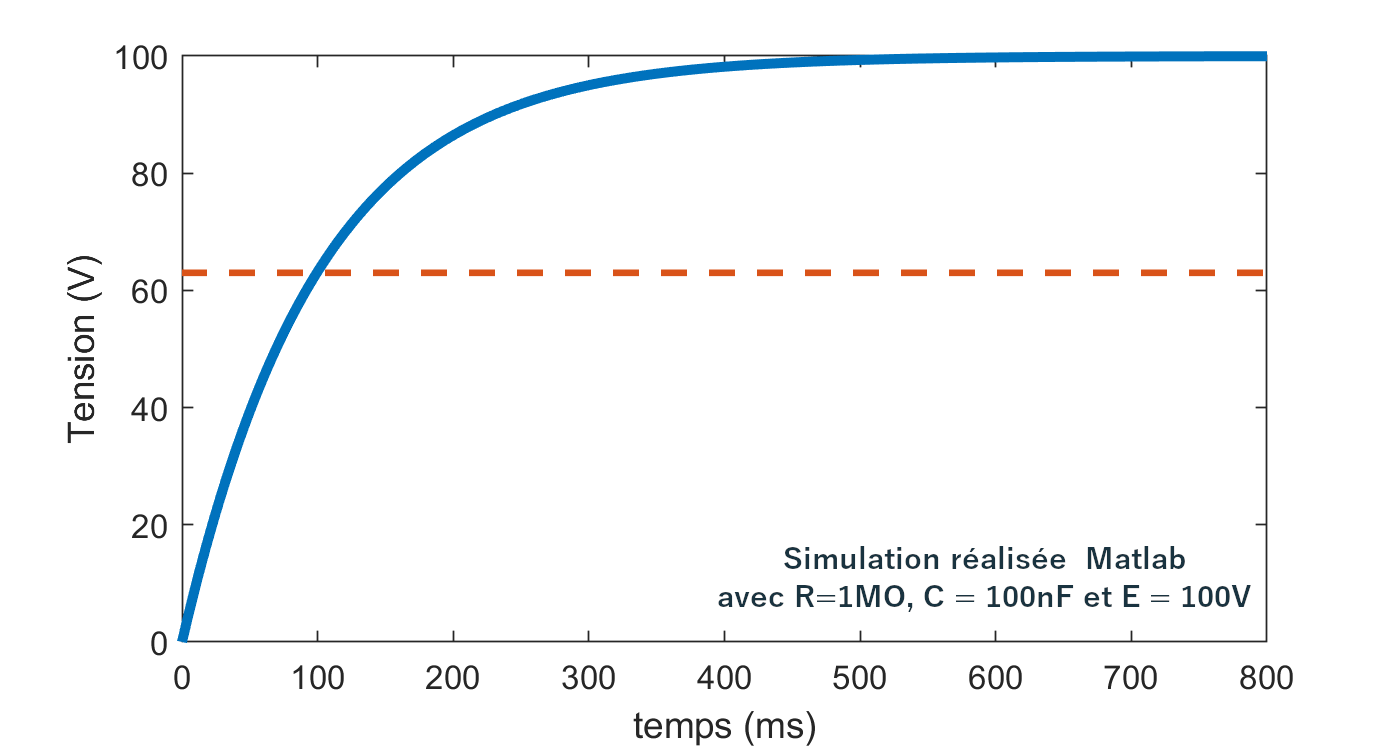
\includegraphics[width=11cm]{images/syst_ordre1_003_a_corr.png}
\end{center}

\centerline {\rule{.5\linewidth}{.25pt}} % Horizontal line

\textbf{Question 3}

Pour mesurer la réponse indicielle (ou réponse à un échelon) de ce circuit, il faut utiliser : 
\begin{itemize}
	\item un générateur de signaux basse fréquence (GBF), appliquant un signal carré de grande période ($T >> R \cdot C$) et d'amplitude d'environ $1\operatorname{V}$ sur l'entrée $V_e(t)$ ;
	\item un oscilloscope permettant de visualiser à la fois $V_e(t)$ (canal 1 et synchronisé sur ce signal) et $V_s(t)$.
\end{itemize}

\newpage
%%%%%%%%%%%%%%%%%%%%%%%%%%%%%%%%%%%%%%%%%%%%%%%%%%%%%%%
\subsection{Exercice 4 - Filtre analogique d'ordre 1}

On reprend le schéma de l'exercice précédent (exercice 3), mais cette fois-ci, nous nous plaçons dans un \textbf{régime harmonique}. Ce circuit est alors alimenté par une source de tension sinusoïdale de pulsation $\omega_0$. On prendra $R = 1\operatorname{M\Omega}$ et $C = 100\operatorname{nF}$.

\begin{enumerate}
	\item Déterminez la \textbf{fonction de transfert} $T( j\omega ) = V_s / V_e$ en fonction de la pulsation et des éléments du montage.
		
	\item Déduisez la \textbf{pulsation de coupure} $\omega_0$ de $T( j\omega )$ et le \textbf{gain dans la bande-passante} en fonction des éléments du montage.

	\item Tracez le \textbf{diagramme de Bode} du gain et de la phase en fonction de la pulsation.

	\medskip
	
	On réalise la réponse en fréquence de ce système expérimentalement à l'aide d'un générateur de fonction ($R_s = 50\operatorname{\Omega}$) et d'un oscilloscope numérique ($R_e = 1\operatorname{M\Omega}$).
	
	Après analyse, nous obtenons une fréquence caractéristique $\omega_c = 20\operatorname{rd/s}$ et une amplification dans la bande passante de 0.5.
	
	\item Proposez une explication à ces résultats.
	
	\medskip
	
	\item On met deux étages de ce type en \textbf{cascade}. Quelle est la fonction de transfert alors obtenue ?

\end{enumerate}


\subsection*{Réponse}

%%%%%%%%%%%%%%%%%%%
\textbf{Question 1}

En appliquant un seul signal sinusoïdal sur ce circuit, on peut alors se placer en régime harmonique et ainsi utiliser les notations complexes. En régime harmonique, l'ensemble des lois fondamentales de la physique peuvent s'appliquer : loi des mailles, loi d'Ohm, superposition...

Ainsi, on a $V_E = R \cdot I + Z_C \cdot I$ avec $Z_C = \frac{1}{j \cdot R \cdot C \cdot \omega}$

On obtient alors : $$I = \frac{j \cdot C \cdot \omega}{1 + j \cdot R \cdot C \cdot \omega} \cdot V_E$$

On a : $V_S = Z_C \cdot I$.

On obtient alors la relation suivante : $$V_S = \frac{1}{1 + j \cdot R \cdot C \cdot \omega} \cdot V_E$$

Ainsi, la fonction de transfert que l'on obtient est la suivante :

$$T(j\cdot\omega) = \frac{V_S}{V_E} = \frac{1}{1 + j \cdot R \cdot C \cdot \omega}$$

\centerline {\rule{.5\linewidth}{.25pt}} % Horizontal line
%%%%%%%%%%%%%%%%%%%
\textbf{Question 2}

On peut alors mettre cette expression sous la forme normalisée d'un système passe-bas du premier ordre : $T(j\cdot\omega) = \frac{T_0}{1 + j \cdot \frac{\omega}{\omega_0}}$. 

On obtient par identification à l'expression obtenue précédemment : $\omega_0 = \frac{1}{R \cdot C}$ et $T_0 = 1$.

L'application numérique donne $\omega_0 = 10\operatorname{rd/s}$ soit une fréquence $f_0 = 1.59\operatorname{Hz}$.


\centerline {\rule{.5\linewidth}{.25pt}} % Horizontal line
%%%%%%%%%%%%%%%%%%%
\textbf{Question 3}

Pour tracer le diagramme de Bode de ce circuit, on s'intéresse au module de la fonction de transfert et à la phase de celle-ci.

Pour simplifier les calculs par la suite, on préfère utiliser le gain (en dB) de cette fonction de transfert : $G = 20 \cdot \log{}(\lvert T \rvert)$

On obtient alors le diagramme de Bode suivant :

\begin{center}
	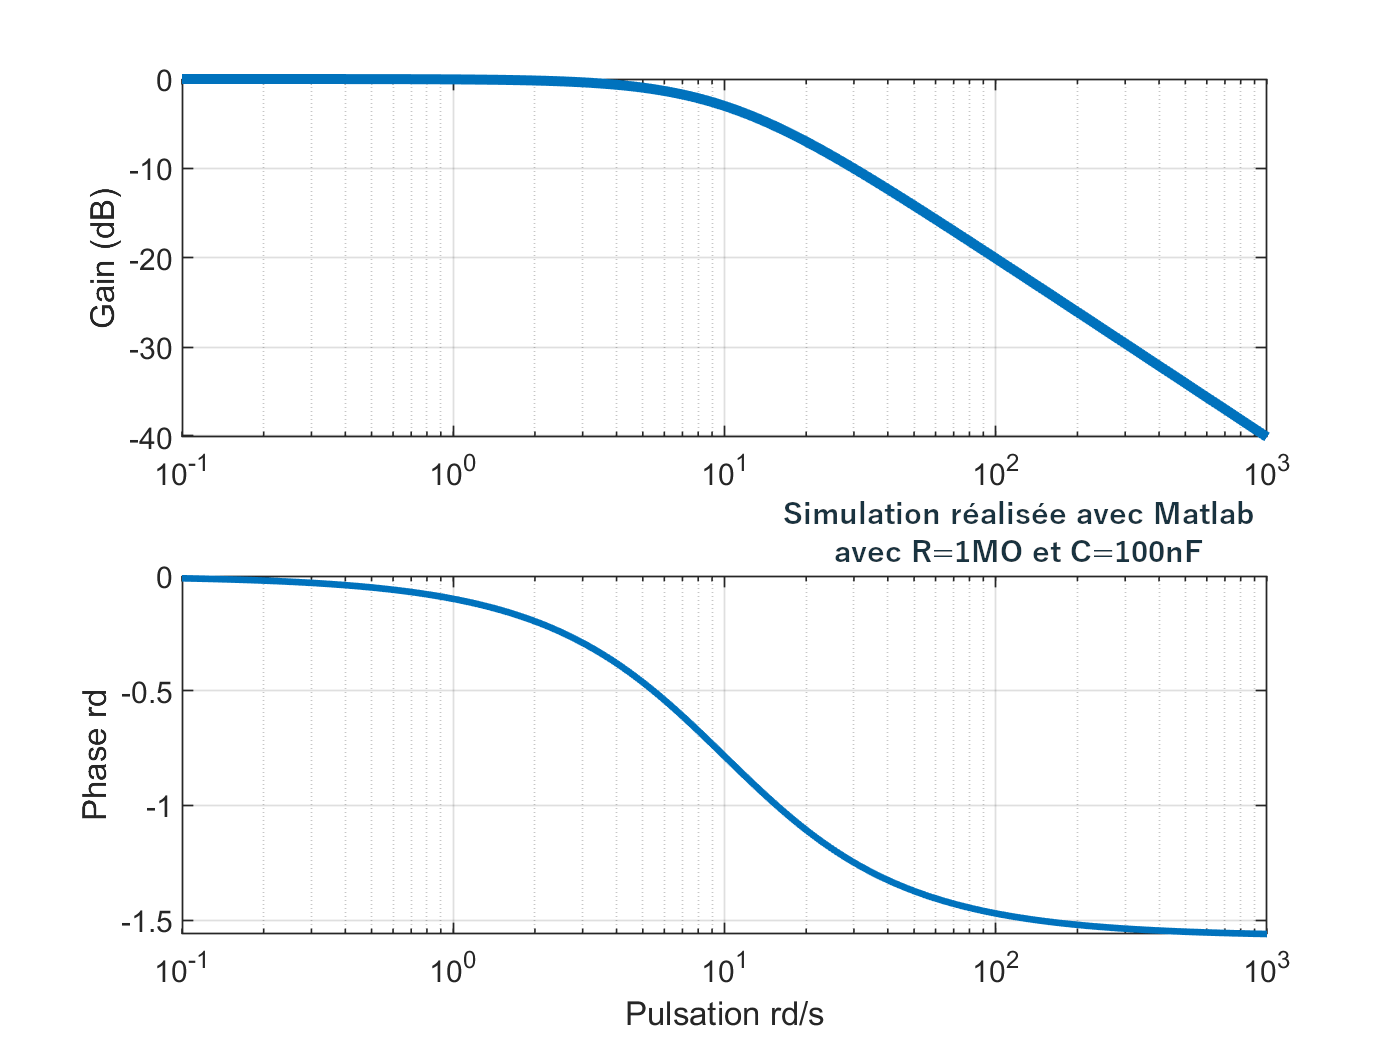
\includegraphics[width=11cm]{images/syst_ordre1_003_b_corr.png}
\end{center}

\textbf{Complément d'informations}

La \textbf{réponse fréquentielle} $H(f) = V_S(f) / V_E(f)$ d'un système permet de connaitre, \textbf{quelque soit la fréquence $f$ du signal d'entrée} : 
\begin{itemize}
	\item l'\textbf{amplitude du signal de sortie} en fonction de celle du signal d'entrée,
	\item le déphasage du signal de sortie par rapport au signal d'entrée.
\end{itemize}

Il est \textbf{théoriquement nécessaire de tester l'ensemble des fréquences du spectre} et de mesurer l'amplitude du signal de sortie et du signal d'entrée ainsi que la phase entre ces deux signaux.

\medskip

\textbf{Mais quel signal faut-il pour réaliser ces mesures ?}

On cherche à mesurer $H(f)$ (dans l'\textbf{espace des fréquences}) pour toutes les fréquence $f$ disponibles. Cependant, nous ne pouvons effectuer nos relevés que dans l'\textbf{espace temporel}. Il serait donc intéressant d'utiliser un signal de fréquence unique $f_0$ tel que la transformée de Fourier de ce signal permette d'obtenir $H(f_0)$ (ou une image de $H(f_0)$). 

On rappelle que $V_S(f) = H(f) \cdot V_E(f)$ dans l'espace fréquentiel, et $v_s(t) = h(t) \ast v_e(t)$ dans l'espace temporel.

\medskip

Si $v_e(t) = A \cdot \sin{}(2 \cdot \pi \cdot f \cdot t)$, alors sa transformée de Fourier vaut : $V_E(f) = \frac{A}{2} \cdot (\delta(-f_0) + \delta(f_0)) $

Ainsi, on obtient en sortie du système : $V_S(f) = H(f) \cdot A \cdot \delta(f_0) = A \cdot H(f_0)$

\centerline {\rule{.5\linewidth}{.25pt}} % Horizontal line
%%%%%%%%%%%%%%%%%%%
\textbf{Question 4} 
	
Les appareils d'instrumentation permettant de réaliser les mesures (ici un GBF et un oscilloscope) ne sont pas parfaits. Il est alors possible de modéliser le montage de la façon suivante :

\begin{center}
	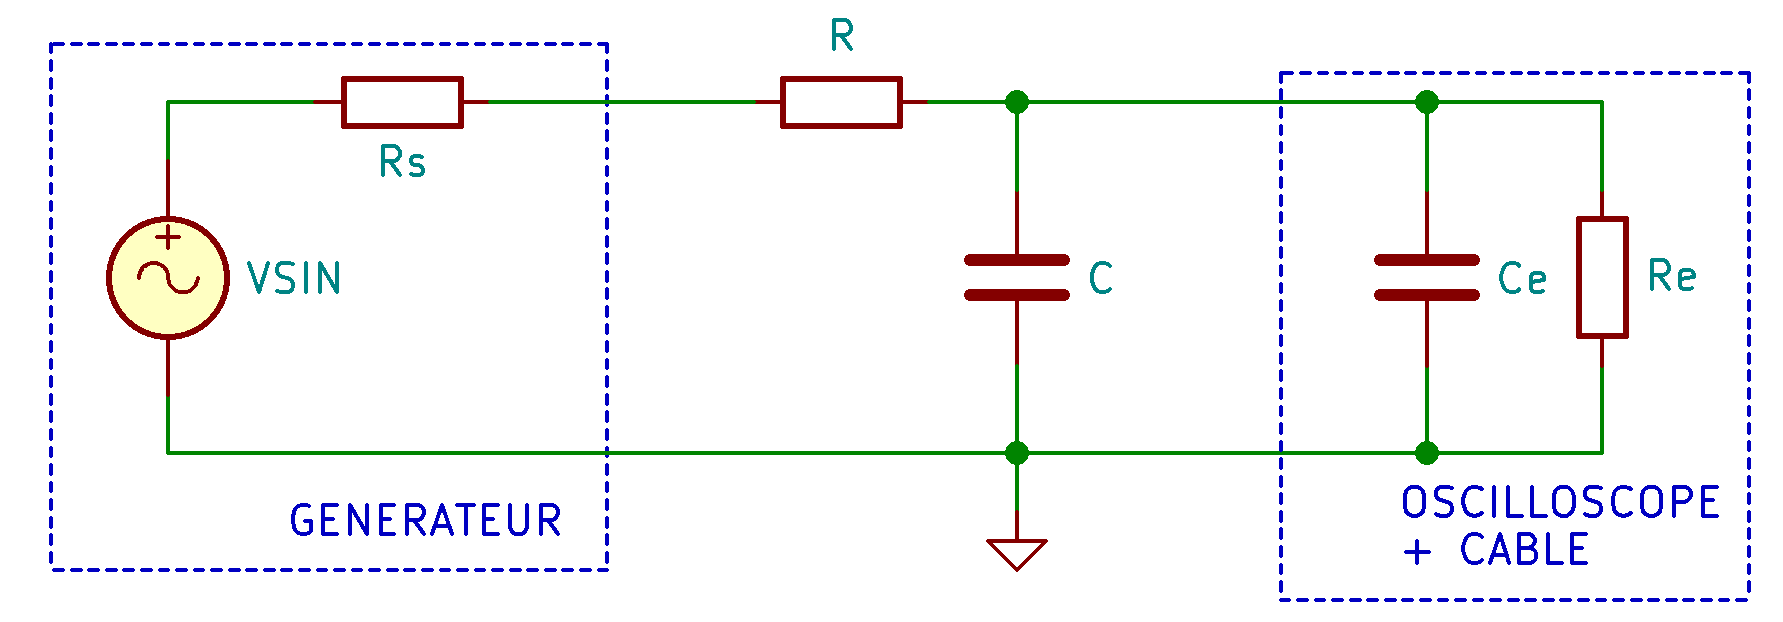
\includegraphics[width=11cm]{images/caract_002_corr.png}
\end{center}

Côté GBF, la tension appliquée (et paramètrée) par le GBF n'est pas tout à fait $V_e$. En effet, l'impédance de sortie du générateur n'est pas nulle (comme elle devrait l'être idéalement). On peut la négliger dans la plupart des cas, car cette dernière vaut en général $50\Omega$.

Côté oscilloscope, nous allons nous intéresser à son impédance d'entrée. Elle est la plupart des cas de $1M\Omega$.

Si on reprend le calcul de la fonction de transfert en prenant en compte l'impédance d'entrée $R_e$ de l'oscilloscope, on obtient alors : 

$$\frac{V_S}{V_e} = \frac{Z_q}{Z_q + R}$$ avec $Z_q = R_e // C = \frac{R_e}{1 + j \cdot R_e \cdot C \cdot \omega}$.

Après simplification, on obtient : 

$$\frac{V_S}{V_e} = \frac{R_e}{R + R_e} \cdot \frac{1}{1 + j \cdot \frac{R \cdot R_e}{R + R_e} \cdot C \cdot \omega}$$

Par identification avec l'expression normalisée d'un filtre du premier ordre, on obtient : $T_0 = \frac{R_e}{R + R_e}$ et $\omega_0 = \frac{R + R_e}{R \cdot R_e \cdot C}$.

\centerline {\rule{.5\linewidth}{.25pt}} % Horizontal line
%%%%%%%%%%%%%%%%%%%
\textbf{Question 5} 

On appelera $V_{S1}$ la sortie du premier étage et $V_{S2}$ celle du second étage.

$V_{S2} = V_{S1} \cdot \frac{1}{1 + j \cdot R \cdot C \cdot \omega}$ (d'après les questions précédentes).

Pour calculer la tension $V_{S1}$, on peut utiliser le théorème de Millman.

On obtient alors : $$V_{S1} = \frac{\frac{V_e}{R} + \frac{V_{S2}}{R}}{\frac{2}{R} + j \cdot C \cdot \omega}$$

Après simplification, on obtient : $$\frac{V_{S2}}{V_e} = \frac{1}{(1 + j \cdot R \cdot C \cdot \omega) \cdot (2 + j \cdot R \cdot C \cdot \omega) - 1}$$

\medskip

Cette fonction de transfert est différente de $T(j \omega)^2 = (\frac{1}{1 + j \cdot R \cdot C \cdot \omega})^2$. La simulation suivante permet de comparer les 3 fonctions de transfert suivantes : celle du premier ordre, celle de la mise en cascade et celle du premier ordre au carré.

\begin{center}
	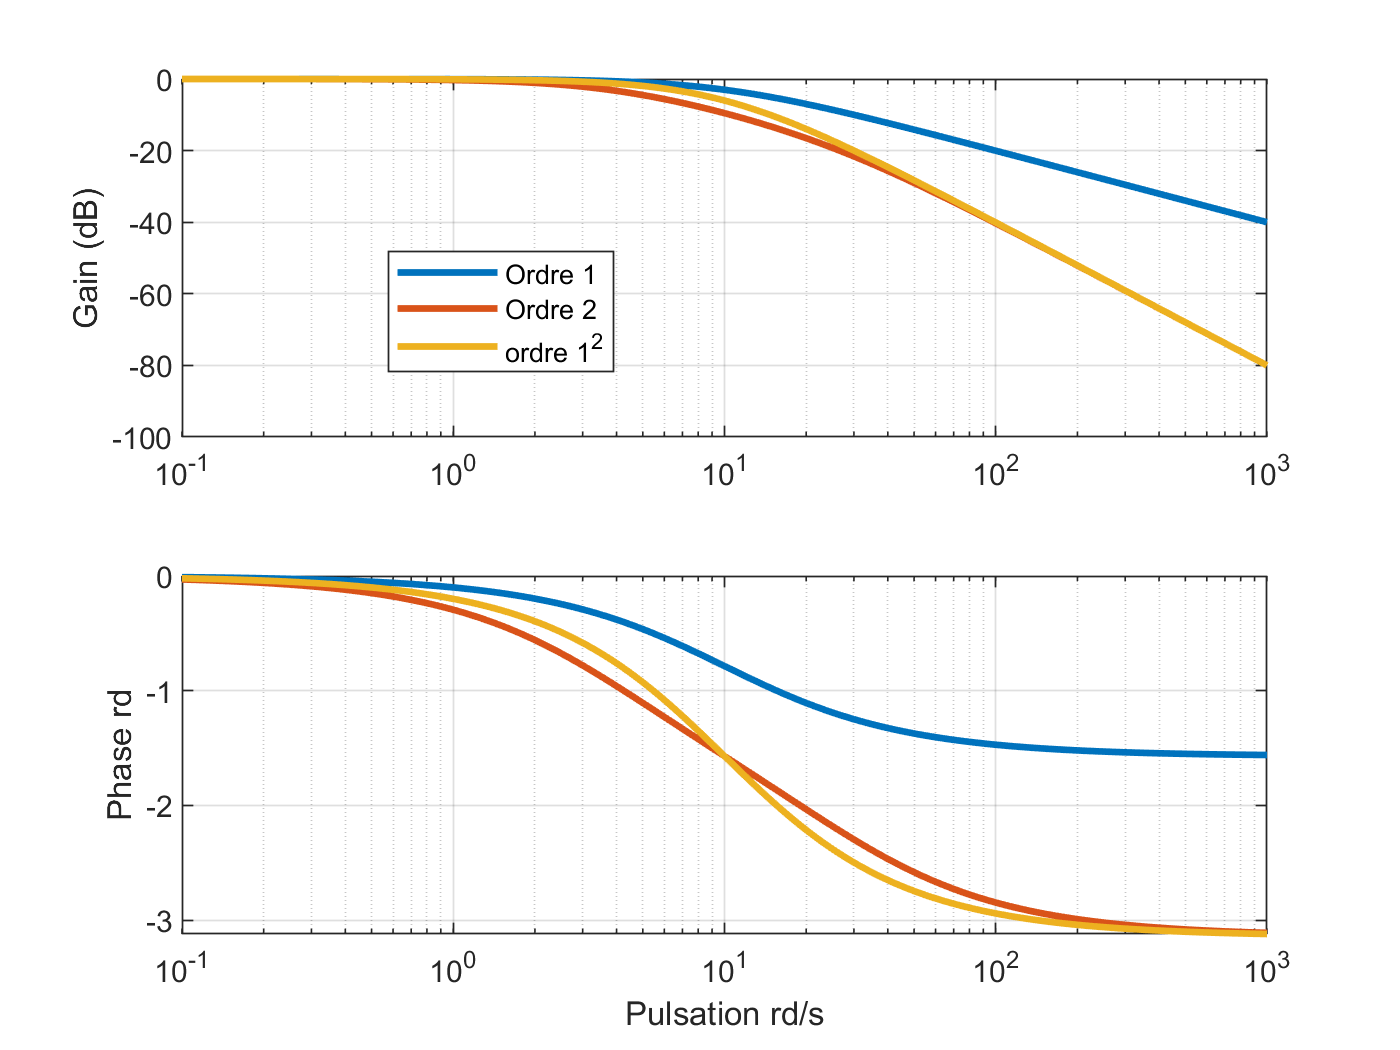
\includegraphics[width=8cm]{images/syst_ordre1_004_b_corr.png}
\end{center}

%%%%%%%%%%%%%%%%%%%%%%%%%%%%%%%%%%%%%%%%%%%%%%%%%%%%%%%